\section{Linear Regression}\label{linear-resression}
\framecard{\insertsection}
\subsection{Basic Concepts of Curve Fitting}

%
%

\subsection{Bayesian Curve Fitting}\label{bayesian-curve-fitting}
\begin{frame}{\insertsubsection}
	\visible<1->{So, we'll start to look the regression with a statistical approach. To encourage you, let's take the sentence.}
	\visible<2>{\vspace{1.5em}
		\begin{block}{Sentence}
		\textit{If we could update the \textbf{\textcolor{red}{regression weights}} as we acquire some new values of the experiment?}
		\end{block}
   		     }
\end{frame}

\begin{frame}{\insertsubsection}
	\visible<1->{Let's take a look again at the Bayes Theorem}
	
	\visible<2->{
	\begin{block}{Bayes Theorem}{
			\begin{equation}\label{bayes_theorem}
				\visible<2->{ p(\mathbf{w}|\mathcal{D}) = \frac{p(\mathcal{D}| \mathbf{w}) \overbrace{ p(\mathbf{w})}^{\mathclap{\text{the weights probability}}}} { \underbrace{ p(\mathcal{D})}_{\mathclap{\text{the data probability}}}} } 
			\end{equation}
			}
	\end{block}
	\visible<3->{So, if\textbf{ we have the probability} of the data, we'll could estimate the\textbf{ future weights}.}
	\visible<4>{\centering\textbf{\textcolor{red}{But, how?}}}
	}
\end{frame}

\begin{frame}{\insertsubsection}
	\visible<1->{Taking some steps back, let's re-visit the \textbf{Curve Fitting}. There, the strategy was minimize the error function.\vspace{1.5em} \\}
	\visible<2->{Now we'll try to view the same problem with a \textit{probabilistic perspective}. We're trying to make predictions for the target value $\mathbf{t}$ given some new values of $x$.\vspace{1.5em} \\}
	\visible<3->{A good ideia is to express our target values $\mathbf{t}$ in terms of \textbf{gaussians distributions} with the mean equals to $y(x,\mathbf{w})$.}
\end{frame}

\begin{frame}{\insertsubsection}
	\begin{figure}
		\label{fig:schematic-gaussian-distribution}
		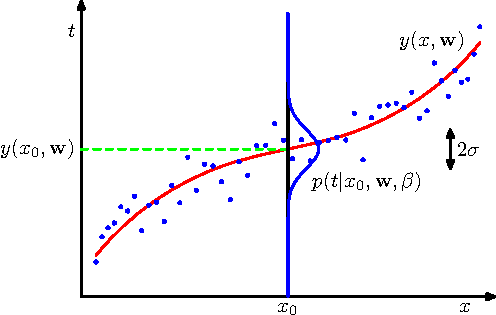
\includegraphics[totalheight=0.6\textheight]{Figure1c16.pdf}
		\caption{Schematic of the polynomial function $y(x,\mathbf{w})$ and the gaussian distribution $p$.}

	\end{figure}
\end{frame}

\begin{frame}{\insertsubsection}
	By the \ref{fig:schematic-gaussian-distribution}, we assume the relation
	\visible<2->{
	\begin{equation}
		p(t|x,\mathbf{w},\beta) = \mathcal{N}(t|y(x,\mathbf{w}),\beta^{-1})
	\end{equation}}
	\visible<3->{and then, assume that the training data $\{ \mathbf{x}, \mathbf{t} \}$ is indenpendent and identically distributed (i.i.d.) and put on \textbf{product form}, i.e. the joint probability is}
	\begin{align} \visible<3->{
		p( \mathbf{t}| \mathbf{x}, \mathbf{w}, \beta) &= \mathcal{N}(t_0|y(x_1, \mathbf{w}), \beta^{-1}) \cap \mathcal{N}(t_n|y(x_0, \mathbf{w}), \beta^{-1}) ... \cap \mathcal{N}(t_n|y(x_0, \mathbf{w}), \beta^{-1}) }\\ 
		\visible<4->{
		&=\prod^N_{n=1} \mathcal{N}(t_n|y(x_n, \mathbf{w}), \beta^{-1})
		}
	\end{align}
	\visible<4->{
	regarding that $\beta^{-1} = \sigma^2$.}
\end{frame}

\begin{frame}{\insertsubsection}
	And we'll have a function to maximize if we apply the logarithm function to $p$, so 
	\visible<2->{
	\begin{equation}
		\ln \left( p( \mathbf{t}| \mathbf{x}, \mathbf{w}, \beta) \right) = \sum^N_{n=1} \ln \left( \mathcal{N}(t_n|y(x_n, \mathbf{w}), \beta^{-1}) \right)
	\end{equation}}
	\visible<3->{
	Applying the \textbf{Gaussian distribution} (see \ref{eq:gaussian-distribution}) will result
	\begin{equation}
		\ln \left( p( \mathbf{t}| \mathbf{x}, \mathbf{w}, \beta) \right) = -\frac{\beta}{2} \sum^N_{n=1} \left\{ y(x_n,\mathbf{w} -t_n ) \right\}^2 + \frac{N}{2}\ln (\beta) - \frac{N}{2} \ln (2 \pi)
	\end{equation}
	}
\end{frame}

\begin{frame}{\insertsubsection}
	And taking the derivatives with respect to $\beta$ to minimize the error
	
		\begin{align}
		\visible<2->{
			\frac{\partial}{\partial \beta}\ln \left( p( \mathbf{t}| \mathbf{x}, \mathbf{w}, \beta) \right) &=0 } \\
		\visible<3->{
			 -\frac{1}{2} \sum^N_{n=1} \left\{ y(x_n,\mathbf{w} -t_n ) \right\}^2 + \frac{N}{2}\frac{1}{\beta} &= 0 \\  }
		\visible<4->{
			 \frac{1}{N} \sum^N_{n=1} \left\{ y(x_n,\mathbf{w} -t_n ) \right\}^2  &= \frac{1}{\beta_{ML}}  }
		\end{align}
	\visible<4->{
	Where $\beta_{ML}$ is the maximum likelihood.}

\end{frame}

%\begin{frame}{Title}
%  $
%    blah =
%    \only<1>{blah}
%    \only<2>{result}
%    \visible<1>{%
%      =
%      \begin{cases}
%          blah \\ 
%          blah
%        \end{cases}
%      }
%    $
%\end{frame}